\definecolor{darkgreen}{rgb}{0,.6,0}
  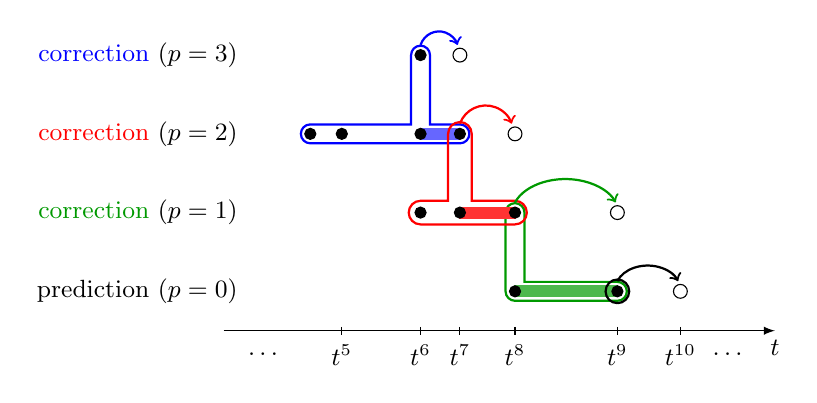
\begin{tikzpicture}[scale=1.0]
    % background grid
    %\draw[step=.2,gray,very thin] (-2.3,-.35) grid (4.4,3.4);

    % \tikzstyle{my style}=[draw=#1,fill=#1!20]
    \tikzstyle{dropline_style}=[densely dotted,thin]

%    \draw[shift={(0.5,2)},dropline_style]  (0,-0.2) -- ++(0,-0.8);
%    \draw[shift={(1.2,2)},dropline_style]  (0,-0.2) -- ++(0,-0.8);

%    \draw[shift={(0.5,3)},dropline_style]  (0,-0.2) -- ++(0,-0.8);
%    \draw[shift={(0,3)},dropline_style] (0,-0.2) -- ++(0,-0.8);

%    \draw[shift={(2.5,1)},dropline_style]  (0,-0.2) -- ++(0,-0.8);
%    \draw[shift={(1.2,1)},dropline_style]  (0,-0.2) -- ++(0,-0.8);


    %\foreach \x/\xtext in {-1, -0.5/-\frac{1}{2}, 1}
    %\draw (\x cm,1pt) -- (\x cm,-1pt) node[anchor=north] {$\xtext$};

    \draw (-2.2, 0) node[left] {\small prediction ($p=0$)};
    %\foreach \y in {1,2,3}
    %  \draw (-2.2, \y) node[left] {\small correction ($p=\y$)};
    \draw (-2.2, 1) node[left] {\small {\color{darkgreen}correction} ($p=1$)};
    \draw (-2.2, 2) node[left] {\small {\color{red}correction} ($p=2$)};
    \draw (-2.2, 3) node[left] {\small {\color{blue}correction} ($p=3$)};

    % position of the time-line
    \def\y{-0.5}
    \draw [-latex] (-2.5,\y) -- (4.5,\y);

    % vertical time grid lines
    %\draw[shift={(-1.4,\y)},dropline_style]  (0,0) -- ++(0,3.5);
    %\draw[shift={(-1,  \y)},dropline_style]  (0,0) -- ++(0,3.5);
    %\draw[shift={(0,   \y)},dropline_style]  (0,0) -- ++(0,3.5);
    %\draw[shift={(0.5, \y)},dropline_style]  (0,0) -- ++(0,3.5);
    %\draw[shift={(1.2, \y)},dropline_style]  (0,0) -- ++(0,3.5);
    %\draw[shift={(2.5, \y)},dropline_style]  (0,0) -- ++(0,3.5);
    %\draw[shift={(3.3, \y)},dropline_style]  (0,0) -- ++(0,3.5);

    \def\tick{0.05}
    \draw (4.5,\y) node[below] {\small $t$};
    \draw (-2,\y) node[below] {\small \phantom{t}$\ldots$\phantom{t}};
    \draw (-1,\y) ++(0,\tick) -- ++(0,-2*\tick) node[below] {\small $t^{5}$};
    \draw (0,\y) ++(0,\tick) -- ++(0,-2*\tick) node[below] {\small $t^{6}$};
    \draw (0.5,\y) ++(0,\tick) -- ++(0,-2*\tick) node[below] {\small $t^{7}$};
    \draw (1.2,\y) ++(0,\tick) -- ++(0,-2*\tick) node[below] {\small $t^{8}$};
    \draw (2.5,\y) ++(0,\tick) -- ++(0,-2*\tick) node[below] {\small $t^{9}$};
    \draw (3.3,\y) ++(0,\tick) -- ++(0,-2*\tick) node[below] {\small $t^{10}$};
    \draw (3.9,\y)  node[below] {\small \phantom{t}$\ldots$\phantom{t}};


    % parameters for stencil diagrams
    \def\rad{0.12}
    \def\omr{0.88}   % 1-rad
    \def\intthick{0.068}   % thickness of integral bars


    % stencil for level 3
    \draw
      [shift={(0.5,3)},thick,blue]
      (0,-1-\rad) arc (-90:90:\rad)
      -- ++(-0.5+\rad,0) -- ++(0,\omr)
      arc (0:180:\rad) -- ++(0,-\omr) -- ++(-1.4+\rad,0)
      arc (90:270:\rad) --cycle
    ;

    % integral bar
    \filldraw[blue!60]
      (0, 2)
      ++(0,-\intthick) --
      ++(0, 2*\intthick) --
      ++(0.5, 0) --
      ++(0, -2*\intthick) --cycle
    ;

    % stencil for level 1
    \draw
      [shift={(2.5,1)},thick,darkgreen]
      (0,-1-\rad) arc (-90:90:\rad)
      -- ++(-1.3+\rad,0) -- ++(0,\omr)
      arc (0:180:\rad) -- ++(0,-\omr) -- ++(0,-1*\rad) arc (180:270:\rad)
      --cycle
    ;

    % integral bar
    \filldraw[darkgreen!70]
      (1.2, 0)
      ++(0, -\intthick) --
      ++(0, 2*\intthick) --
      ++(1.3, 0) --
      ++(0, -2*\intthick) --cycle
    ;

    % increase the radius for the remaining stencil diagrams
    \def\rad{0.15}
    \def\omr{0.85}   % 1-rad

    % stencil for level 0
    \draw
      [shift={(2.5,0)},thick,black]
      (0,-\rad) arc (-90:270:\rad)
    ;

    % stencil for level 2
    \draw
      [shift={(1.2,2)},thick,red]
      (0,-1-\rad) arc (-90:90:\rad)
      -- ++(-0.7+\rad,0) -- ++(0,\omr)
      arc (0:180:\rad) -- ++(-0,-\omr) -- ++(-0.5+\rad,0)
      arc (90:270:\rad) --cycle
    ;


    % integral bar
    \filldraw[red!80]
      (0.5, 1)
      ++(0,-\intthick) --
      ++(0, 2*\intthick) --
      ++(0.7, 0) --
      ++(0, -2*\intthick) --cycle
    ;

    % arrows
    \draw [->,thick,blue] (0,3.13) arc (160:20:0.25 and 0.26);
    \draw [->,thick,darkgreen] (1.2,1.13) arc (160:20:0.68 and 0.45);
    \draw [->,thick,black] (2.5,0.13) arc (160:20:0.41 and 0.3);
    \draw [->,thick,red] (0.5,2.13) arc (160:20:0.35 and 0.35);

    % filled dots
    \foreach \xy in {
      (1.2,0),(2.5,0),
      (0,1),(0.5,1),(1.2,1),
      (-1.4,2),(-1,2),(0,2),(0.5,2),
      (0,3)
      }
      \filldraw \xy circle (2pt)
    ;
%    %\filldraw[fill=red] \trixy  circle (3.5pt);
%    \def\rad{0.13}
%    \filldraw[fill=white,shift={\trixy}]
%    (0,0) (90:\rad) -- (-150:\rad) -- (-30:\rad) -- cycle;
%    %\draw (\x cm,1pt) -- (\x cm,-1pt) node[anchor=north] {$\xtext$};
%    %\node (N) at
%    %(0,0) [draw, shape=triangle] {$v_0$};


    % hollow dots
    \foreach \xy in { (3.3,0),(2.5,1),(1.2,2),(0.5,3) }
    \filldraw[fill=white] \xy circle (2.5pt);
  \end{tikzpicture}
